\section{Umsetzung des Prototypen emoTrix}
Hier werden Dinge umgesetzt.
\subsection{MockUps}
\subsection{Datenerfassung in Form von Emotionstests}
\subsubsection{GSR-Test}
\subsubsectionauthor{Lukas Seemann}
Die Erfassungsmöglichkeit mit der höchsten Priorität war die Messung der Hautleitfähigkeit mithilfe von EDA- beziehungsweise GSR-Sensoren. Da dies nicht mit im Smartphone enthaltenen Sensoren möglich war, wurde zusätzlich ein Arduino-Mikrocontroller benötigt, um die Messung durchzuführen. Zunächst wird die Entwicklung auf dem Arduino-Board mit allen zusätzlichen Modulen beschrieben. Im Anschluss daran wird thematisiert, wie das Arduino-Board mit der App verbunden wurde. \newline
Für das Projekt wurde ein Arduino UNO R3 Board verwendet. \footcite[Vgl.][]{Ard18} Dieser kann mit Stromzufuhr über ein Netzteil oder per USB betrieben werden. Als Sensor wurde ein GSR Sensor des Grove-Toolkits verwendet\footcite[Vgl.][]{Gro18}, der bereits in Abbildung 5 gezeigt wird. Am Sensor selbst werden die Elektroden für die Finger angebracht. Da ein handelsübliches Arduino UNO R3 Board nicht über den benötigten Anschluss für den Grove GSR-Sensor verfügt, muss zusätzlich noch ein Grove Base Shield angebracht werden. Dieses kann auf das Arduino Board aufgesteckt werden und erweitert es um viele verschiedene Anschlüsse, unter anderem für Sensoren.
\begin{figure}[h]
	\centering
	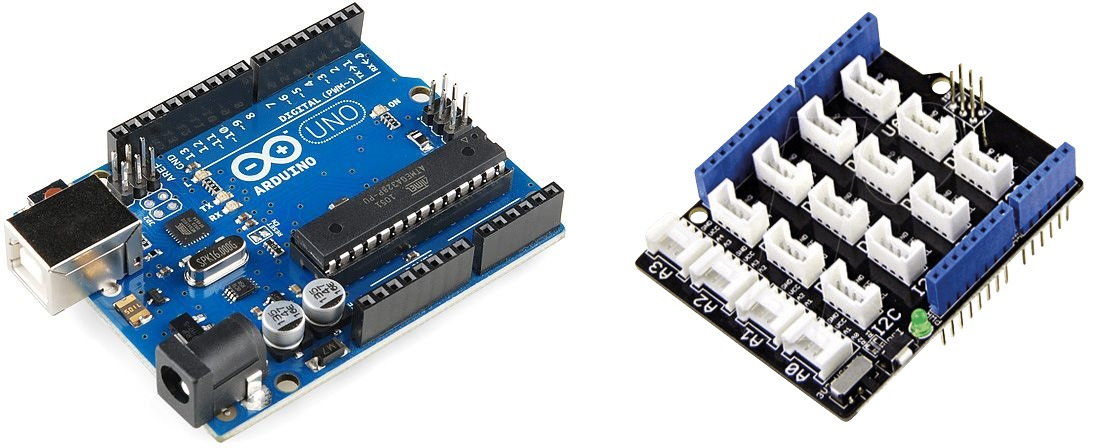
\includegraphics[width=16cm]{Bilder/arduino.jpg}
	\caption[Arduino UNO R3 (links) und Grove Base Shield]{Arduino UNO R3 (links) und Grove Base Shield\footnotemark}
\end{figure}%
\footcitetext[Bilder von:][]{Sou18, Rei18}
\subsection{Auswertung der Testergebnisse}
\subsection{Benutzeroberfläche der App}
